\chapter{Sistema de detección 2D con cámara}
\label{cha:Sistema de detección 2D con cámara}

\begin{FraseCelebre}
  \begin{Frase}
    Texto.
  \end{Frase}
  \begin{Fuente}
    Autor texto
  \end{Fuente}
\end{FraseCelebre}

\noindent
El sistema de visión artificial basado en una fusión sensorial que se ha diseñado, se basa en una primera fase de detección 2D con cámara. Dichas detecciones 2D, serán utilizadas más adelante para realizar una aproximación a la distancia de los diferentes objetos detectados como se presenta en el Capítulo \ref{cha:Propuesta de trabajo}. Requiriendo de un sistema que sea ejecutable en tiempo real con gran precisión en las detecciones, se decide optar por un modelo basado en Deep Learning como es YOLO \cite{YOLOv4}, VGG16 \cite{VGG16} o ResNet \cite{ResNet}.

Estos modelos de detección de objetos 2D no se basan únicamente en las típicas redes totalmente conectadas o \ac{FC}, en las que todas las neuronas de una capa de conectan con todas las neuronas de la siguiente capa, sino que se suelen basar en \ac{CNN} y en técnicas como el aprendizaje por trasferencia o tranfer learning. Dichas técnicas se explicaran a continuación debido a la gran importancia en el diseño y entrenamiento del modelo utilizado.

En cuanto a la elección del modelo con el que trabajar, y que se incorporará al flujo de ejecución del modelo completo de detección 3D, se decanta por el uso de YOLOv5 \cite{YOLOv5}. En el último año, este modelo basado en Deep Learning ha desbancado al resto de detectores 2D debido a su gran precisión en las detecciones, además de la velocidad de inferencia de dichas detecciones, siendo dicho modelo accesible de manera open source en GitHub.

\section{Técnicas de Deep Learning aplicadas a detección 2D}
\label{sec:Técnicas de Deep Learning aplicadas a detección 2D}

Antes de explicar la arquitectura del modelo YOLOv5, se presentan dos técnicas muy utilizadas no solo en este modelo sino en todo el campo de la visión por computador. Por una parte, el tipo de arquitectura más utilizado para modelos de visión basados en cámara como son las \ac{CNN}, y por otra una técnica que permite la trasferencia de conocimiento sobre modelos basados en Deep Learning.

\subsection{Convolutional Neural Networks}
\label{sec:Convolutional Neural Networks}

Las redes neuronales convolucionales o \acl{CNN} se distinguen de otras redes neuronales por su rendimiento superior en modelos que utilizan imágenes y audio. Dichas redes se suelen basar en tres tipos de capas diferentes: las capas convolucionales, las capas de agrupación o pooling layer y las capas \acl{FC} \cite{what_cnn}.

Las capas convolucionales son el bloque principal de las \ac{CNN} y es donde se produce la mayor parte del cálculo en estos modelos. Estas capas requieren de varios componentes, como es la matriz de entrada, un filtro o kernel y la salida o mapa de características. La entrada de una capa convolucional suele ser un vector o tensor de dos dimensiones, en el caso de utilizar una imagen como entrada, en vez de tener una estructura matricial se tienen múltiples matrices que pueden ser procesadas con diferentes kernels. Los kernels son una serie de matrices que extraen las características de las matrices de entrada, por esto mismo se utilizan múltiples kernels sobre una misma matriz para obtener información diferente en función del filtro o kernel utilizado.

\begin{figure}[H]
    \centering
    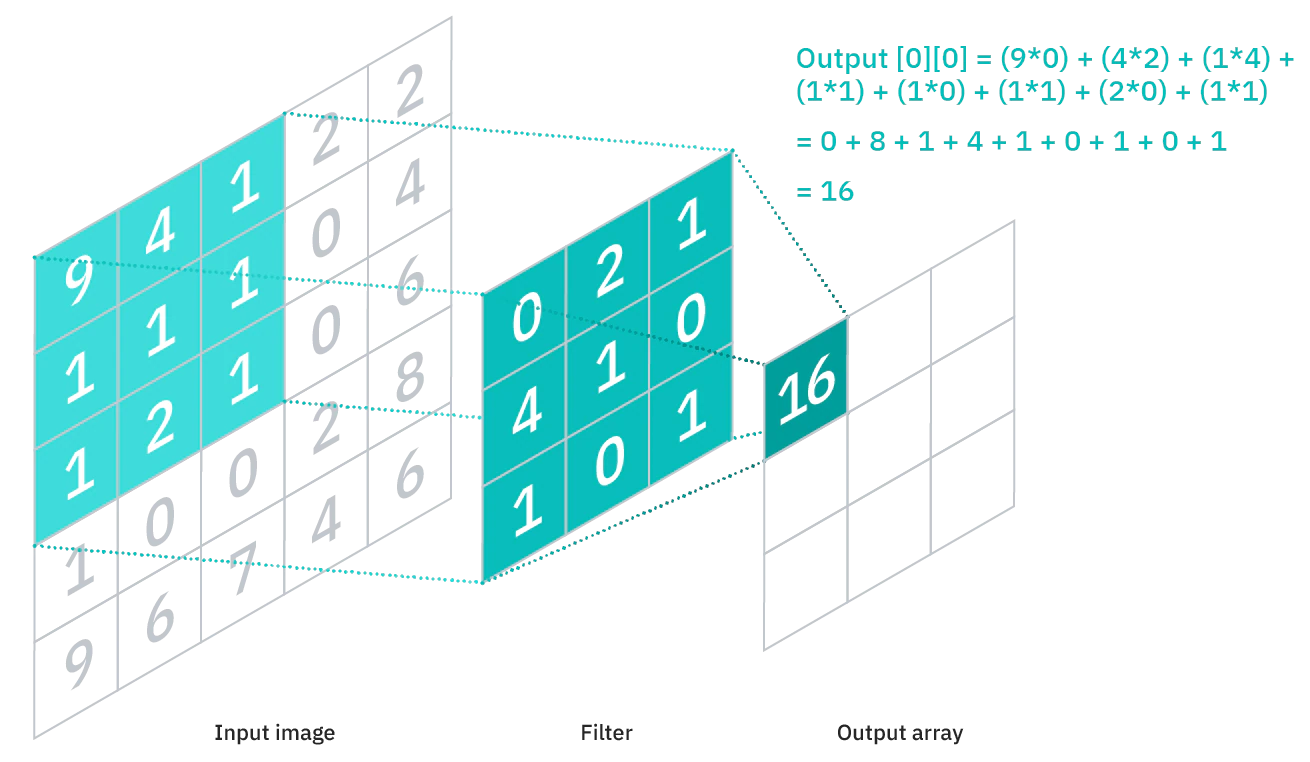
\includegraphics[width=0.6\textwidth]{Book/figures/5_deteccion2d/cnns.png}
    \caption{Operación de multiplicación y acumulación.}
    \label{fig:Operación de multiplicación y acumulación.}
\end{figure}

El mapa de características es obtenido mediante la aplicación de una operación de convolución del kernel sobre la matriz de entrada, para ello se realizan los siguientes pasos: se coloca el kernel sobre una de las regiones de la matriz de entrada y se aplica una operación de multiplicación y acumulación, donde se multiplica elemento a elemento cada uno de las posiciones de cada matriz y posteriormente se suman los valores obtenidos, tal y como se observa en la Figura \ref{fig:Operación de multiplicación y acumulación.}, tras esto se repite la operación sobre cada una de las posiciones donde se puede colocar el kernel en la matriz hasta formar una nueva matriz.

Dicho mapa de características si no se ha realizado ninguna modificación a los diferentes pasos presentados, suele ser más pequeña que la matriz de entrada. Este paso de la operación de convolución en si mismo requiere de la elección de muchas características como: la decisión de añadir un 'borde' a la imagen para aumentar el tamaño de la matriz de salida, también llamado padding; por otra parte, también se puede modificar el numero de celdas desplazadas por el kernel sobre la matriz de entrada produciendo un mapa de características de menor tamaño, este parámetro es llamado stride; por último, el uso de un mayor número de kernels permite la extracción de más cantidad de información de la matriz de entrada, pero esto resulta en tiempos de ejecución más lentos.

\begin{figure}[H]
    \centering
    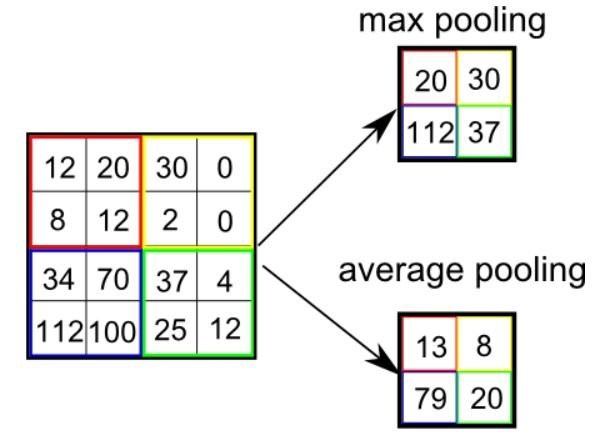
\includegraphics[width=0.3\textwidth]{Book/figures/5_deteccion2d/pooling.jpeg}
    \caption{Max pooling y average pooling.}
    \label{fig:Max pooling y average pooling.}
\end{figure}

El segundo de los tipos de capas más utilizados en las redes neuronales convolucionales son las pooling layers, estas capas son utilizadas para la reducción del tiempo de computo de este tipo de arquitectura. Para lograr dicha característica, las pooling layer realizan una operación dada sobre cada una de la regiones definidas de una matriz. Las operaciones típicamente utilizadas son la obtención del valor máximo y la media, también llamadas max pooling y average pooling. Para la aplicación de estas técnicas se suele utilizar un tamaño de región fijo en toda la matriz de 2x2, pero este valor es configurable según se requiera. Un ejemplo de esta técnica que muestra que muestra su efectividad en la reducción de la dimensión de la matriz de entrada se muestra en la Figura \ref{fig:Max pooling y average pooling.}.

Por último, la tercera técnica más utilizada dentro de las redes neuronales convolucionales son las capas \acl{FC}, dichas capas son la base de las redes neuronales. Dicha capa realiza una conexión de todas las neuronas de una capa con las neuronas de la siguiente capa. Este tipo de capa suele ser utilizado a la salida de las redes neuronales debido a su capacidad de utilizar cualquier tipo de entrada, procesarlo y obtener la salida requerida.

\begin{figure}[H]
    \centering
    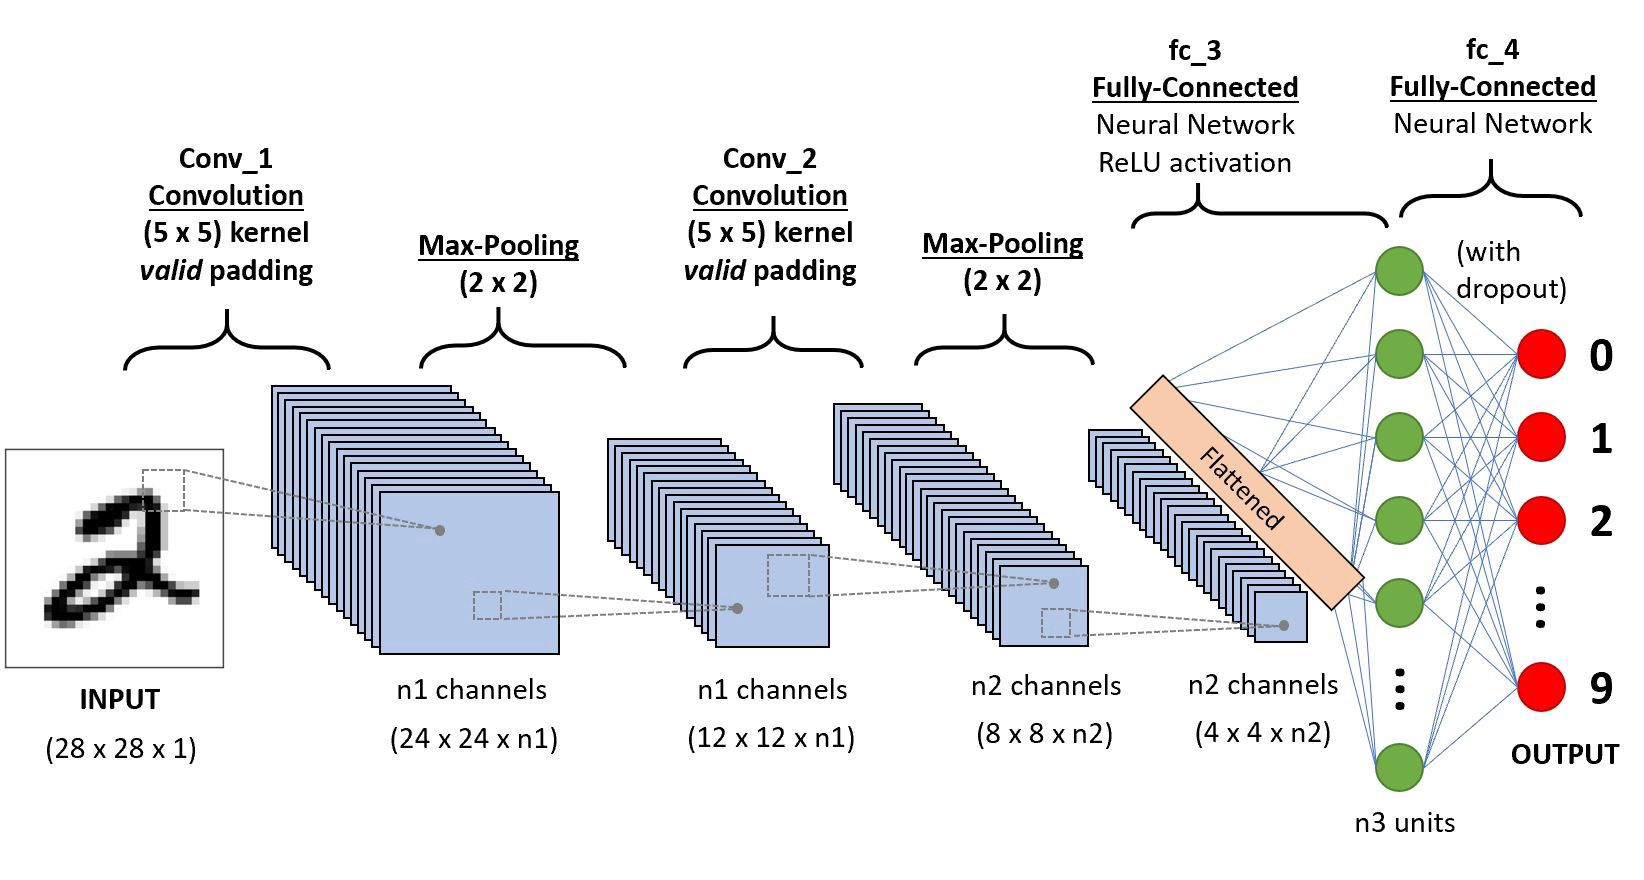
\includegraphics[width=0.7\textwidth]{Book/figures/5_deteccion2d/CNN.jpeg}
    \caption{Red neuronal convolucional.}
    \label{fig:Red neuronal convolucional.}
\end{figure}

La estructura de las \ac{CNN} se utiliza en gran parte de los modelos de visión artificial, esto se observa en el Capítulo \ref{cha:Estado del arte en técnicas de fusión sensorial}, donde gran parte de los modelos de fusión sensorial utilizan todas estas capas. En cuanto al uso de las \ac{CNN}, se pueden aplicar en su forma más simple para la clasificación de imágenes entre otras aplicaciones como se muestra en la Figura \ref{fig:Red neuronal convolucional.}.

\subsection{Transfer learning}
\label{sec:Transfer learning}

El aprendizaje por transferencia o transfer learning es la reutilización de un modelo preentrenado en un nuevo problema. Actualmente es muy popular en modelos basados en Deep Learning porque permite el entrenamiento de redes neuronales con relativamente pocos datos \cite{what_tl}. 

Utilizando el transfer learning, el conocimiento de un modelo de \ac{ML} ya entrenado se aplica a un problema diferente pero relacionado. Por ejemplo, en el caso de tener un modelo de traducción de inglés a español, se podría aplicar este conocimiento para el entrenamiento de un modelo que consigue traducir de inglés a chino. Esto es así, ya que los pesos de la red neuronal tienen de forma implícita el conocimiento del idioma inglés y es capaz de pasar a comprender otro idioma de forma más sencilla al no tener que comprender de nuevo dos idiomas.

En el campo de la visión por computador, el transfer learning se realiza mediante el uso de modelos de clasificación o detección preentrenados sobre datasets enormes que son muy difícilmente entrenables sin un hardware con un coste muy elevado, como ocurre con el dataset de ImageNet \cite{ImageNet_dataset} y COCO \cite{COCO_dataset}.

El proyecto de ImageNet consta de la creación de un dataset con más de 1.000 imágenes por cada una de las 22.000 clases que se tienen, para ello, el dataset se compone de más de un millón de bounding boxes 2D anotadas manualmente. Debido en parte a la creación de este dataset en 2012, se produce una gran mejora en las diferentes técnicas de visión artificial basadas en \ac{CNN}, ya que al tratar con tal cantidad de imágenes anotadas no se produce ningún tipo de overfitting. Por otra parte, el dataset de COCO contiene alrededor de 200.000 imágenes anotadas, lo cual lo hace un dataset más pequeño que ImageNet, pero al contrario de dicho dataset, se tienen anotaciones adicionales de segmentación semántica \cite{top_img_datasets}.

Debido a la influencia de estos datasets, hoy en día librerías de Deep Learning como: fastai \cite{fastai}, PyTorch \cite{Pytorch} o TensorFlow \cite{Tensorflow}; permiten el uso de modelos de visión artificial o procesamiento del lenguaje junto con sus pesos preentrenados que pueden ser opcionalmente descargados.

\section{YOLOv5}
\label{sec:YOLOv5}

La quinta versión del modelo \ac{YOLO} es la elegida para la obtención de las detecciones 2D utilizadas en el sistema completo de detección de objetos 3D. Desde la presentación de la primera versión del modelo \ac{YOLO}, se observa como el diseña esta red se centra en la ejecución en tiempo real debido a la obtención de las detecciones en un solo paso, tal y como implica el nombre del modelo ('solo mira una vez').

Debido a la falta de un paper de la última versión de este modelo, la explicación del funcionamiento del modelo se basará en los modelos: YOLOv3 \cite{YOLOv3}, YOLOv4 \cite{YOLOv4} y YOLOv5 \cite{YOLOv5}. En comparación con el enfoque adoptado por los algoritmos de detección de objetos anteriores a \ac{YOLO}, que reutilizan clasificadores para realizar la detección, \ac{YOLO} propone el uso de una red neuronal de extremo a extremo que realiza predicciones de bounding boxes e inferencia de la clase de una sola vez \cite{yolo_comparison}.

\begin{figure}[H]
    \centering
    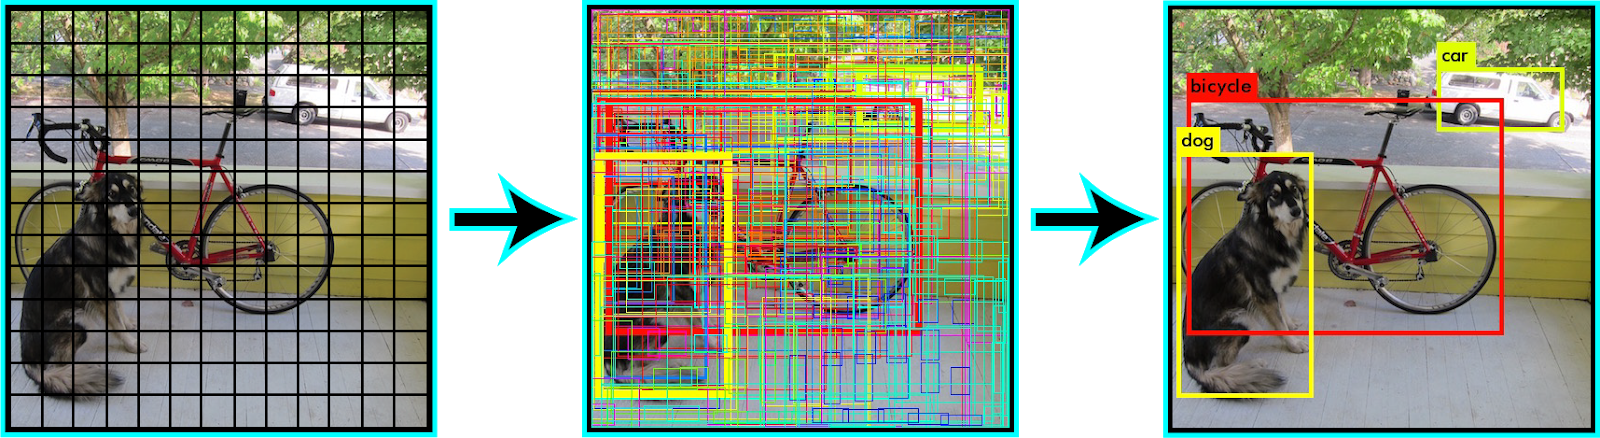
\includegraphics[width=0.9\textwidth]{Book/figures/5_deteccion2d/yolo_example.png}
    \caption{Pasos realizados por YOLO}
    \label{fig:Pasos realizados por YOLO}
\end{figure}

Mientras que algoritmos como Faster R-CNN \cite{Faster_R-CNN} trabajan detectando posibles regiones de interés mediante una \ac{RPN} y luego realizan el reconocimiento en esas regiones por separado, \ac{YOLO} realiza todas sus predicciones con la ayuda de una capa Fully Connected.

El modelo \ac{YOLO} funciona dividiendo la imagen en N cuadrículas, cada una de las cuales tiene una región de igual dimensión. Cada una de estas N cuadrículas es responsable de la detección y localización del objeto que contiene. En consecuencia, estas cuadrículas predicen las coordenadas de la bounding box en relación con las coordenadas de su celda, junto con la clase del objeto y la probabilidad de que el objeto esté presente en la celda. Debido a la gran cantidad de bounding boxes producidas, se aplica el algoritmo \ac{NMS} (presentado en el Algoritmo \ref{alg:Algoritmo NMS}) para reducir las bounding boxes con una probabilidad menor.

\begin{algorithm}[H]
\caption{Algoritmo NMS}\label{alg:Algoritmo NMS}
\SetKwInput{KwInput}{Input}                % Set the Input
\SetKwInput{KwOutput}{Output}              % set the Output
\SetKwBlock{Beginn}{beginn}{ende}
\DontPrintSemicolon
  \KwInput{$B = {b_1,...,b_N}, S = {s_1,...,s_N}, u$\\
  \hspace{33pt}$B$ es la lista con las bounding boxes\\
  \hspace{33pt}$S$ es la lista con la probabilidad de las bounding boxes\\
  \hspace{33pt}$u$ es el ĺímite del algoritmo NMS}
  \Begin{
  $D \gets \{\}$\;
  \While{$B \neq \textit{empty}$}{
  $m \gets \textit{arg max} S$\;
  $M \gets b_m$\;
  $D \gets D \cup M$\;
  $B \gets B - M$\;
  \For{$B_i \in B$}{
  \If{$\textit{IoU} (M,b_i)$}{
    $s_i \gets s_i * (1 - \textit{IoU}(M,b_i))$}
  }
  }
  \Return $D, S$}
\end{algorithm}

Inspirada en la arquitectura de GoogLeNet \cite{GooLeNet}, la arquitectura de \ac{YOLO} tiene un total de 24 capas convolucionales con 2 capas totalmente conectadas al final. Para mejorar la segunda versión de este modelo y poder competir contra modelos como los basados en \ac{SSD} o los ResNet \cite{ResNet} o mode, YOLOv3 utiliza un backbone (capas base de un modelo) con un mayor número de capas para mejorar la capacidad de detección del modelo, de forma adicional se incorpora el uso de skip layers (técnica que se basa en la conexión de una capa con otra posterior) para permitir el uso de características a diferentes niveles en la obtención de las detecciones finales.

YOLOv4 propone la adición de las 'Conexiones Residuales Ponderadas' o Weighted  Residual Connections, la 'Normalización de Mini Lotes Cruzados' o Cross Mini Batch Normalization, las 'Conexiones Parciales Cruzadas' o Cross Stage Partial Connections, el 'Entrenamiento Adversario' o Self Adversarial Training y la Activación Mish ($f(x) = x * \tanh{(\ln{(1+e^x)})}$) como cambios metodológicos entre los métodos modernos de regularización y aumento de datos.

Por último, YOLOv5 es un proyecto open source que consiste en una familia de modelos de detección de objetos y métodos de detección basados en el modelo \ac{YOLO} preentrenado en el dataset de COCO.

\section{Entrenamiento y evaluación de YOLOv5}
\label{sec:Entrenamiento y evaluación de YOLOv5}

La creación del sistema de detección 2D se ha basado en YOLOv5, debido a su velocidad de inferencia y la precisión del modelo. En cuando a la implementación del modelo, se ha utilizado el repositorio git alojado en GitHub de la empresa Ultrlytics. Dicho repositorio permite entrenar, validar e implementar de forma sencilla dicho modelo de obtención de detecciones 2D.

Una de las opciones más importantes que permite el uso de este repositorio es el uso de transfer learning, ya que se pueden utilizar los pesos de la red preentrenada sobre todo el dataset de COCO. En el propio repositorio se observa la Figura \ref{fig:Evaluación de YOLOv5 sobre el dataset de COCO}, donde se ven las diferentes métricas obtenidas sobre dicho dataset con cada una de las versiones que se ofrecen del modelo. Dicha imagen muestra las diferentes versiones: n, s, m, l, x; como se comportan en cuanto a la velocidad de ejecución y el \ac{AP} (métrica que define la precisión de las detecciones como el área bajo la curva PR), en todas ellas se observa una mejora en relación precisión/velocidad respecto al modelo EfficientDet \cite{EfficientDet}.

\begin{figure}[H]
    \centering
    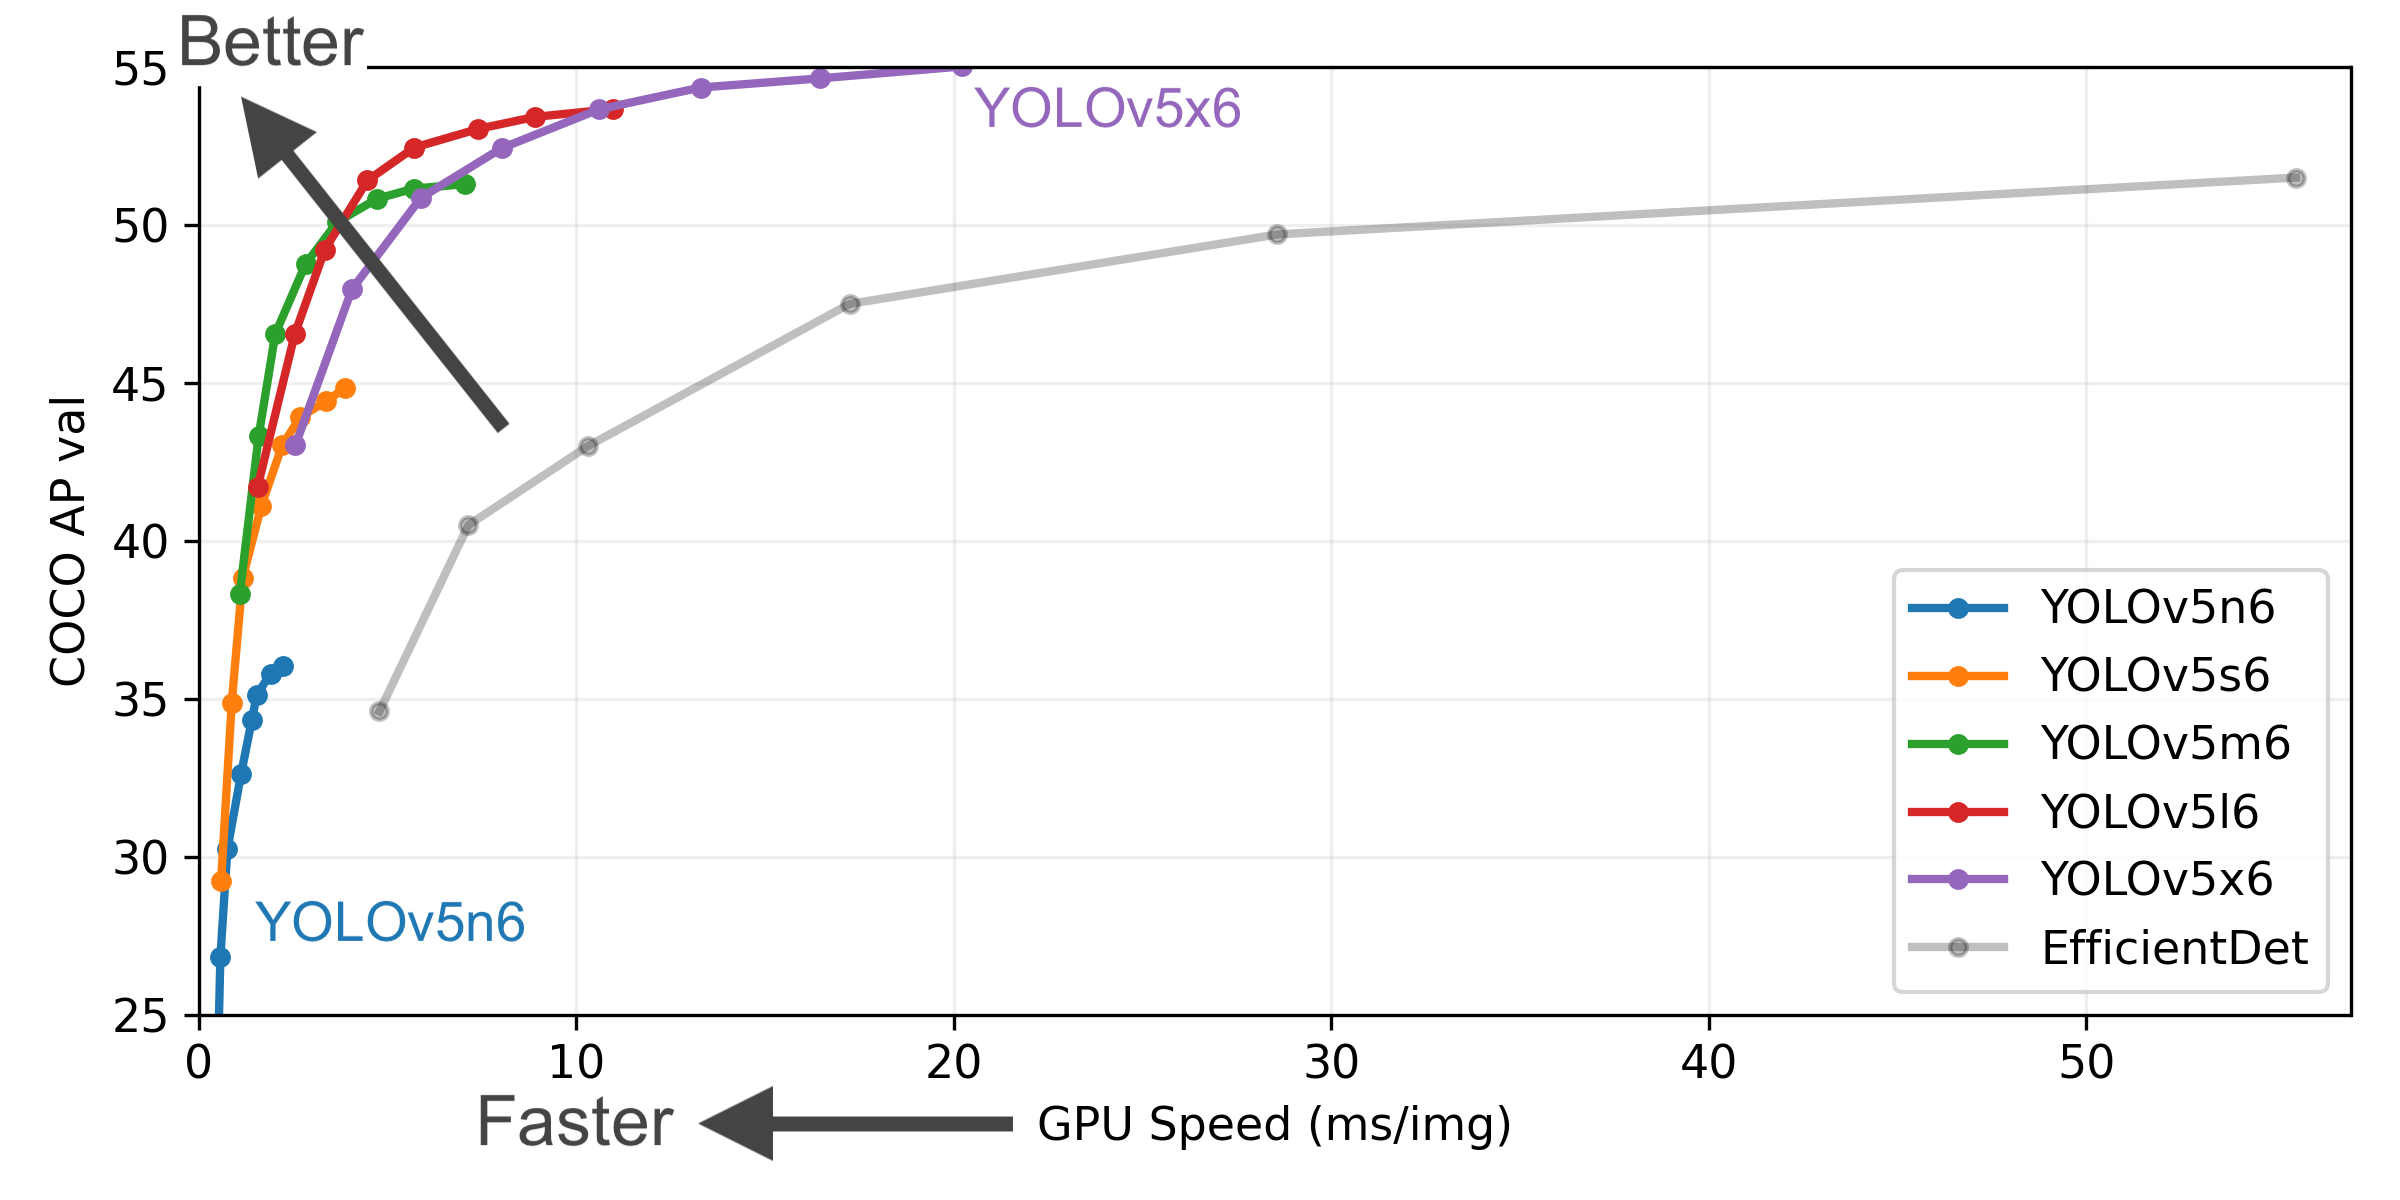
\includegraphics[width=0.7\textwidth]{Book/figures/5_deteccion2d/yolov5_eval.png}
    \caption{Evaluación de YOLOv5 sobre el dataset de COCO}
    \label{fig:Evaluación de YOLOv5 sobre el dataset de COCO}
\end{figure}

El dataset de COCO sobre el que se encuentra entrenado cada una de las versiones del modelo, permite la detección de multitud de clases diferentes, las cuales podrían ser utilizadas sobre el dataset de KITTI, en este caso: coches, peatones y ciclistas. Dentro de COCO se encuentran tres clases muy similares como son: coches, personas y bicicletas; de esta manera no debería ser necesario el entrenamiento de este modelo ya que se podrían utilizar los pesos por defecto, pero se ha observado que estas clases no son lo suficientemente parecidas. Por ejemplo, como fallo principal se ha encontrado como en el caso de KITTI, se requiere la detección de la clase ciclista, mientras que en COCO se tiene a la clase persona y bicicleta, se ha observado como en el caso de detectar a un ciclista en KITTI, el modelo divide la detección entre bicicleta y persona (encima de la bicicleta), esto resulta en un problema para la obtención de las detecciones por lo que se decide entrenar de nuevo este modelo para un mejor ajuste sobre las clases que tiene que ser detectadas. Para ello se utilizará el dataset de KITTI con las bounding boxes 2D del ground-truth 

La implementación de YOLOv5 utilizada se basa en el uso del dataset de COCO, por ello, se ha modificado el dataset de KITTI para que adopte el mismo formato que este dataset ya que tiene una estructura muy similar y se puede realizar de forma muy sencilla.

\begin{table}[H]
\centering
\begin{tabular}{@{}ccccccc@{}}
\toprule
Modelo                   & Fine-tuning & AP coches & AP bicicletas & AP peatón & mAP & Tiempo de inferencia  \\ \midrule
\multirow{2}{*}{YOLOv5s} & No          & 0.912         & 0.630             & 0.709         & 0.750   & \multirow{2}{*}{5.800 ms} \\
                         & Sí          & 0.905         & 0.621             & 0.740         & 0.755   &                       \\
\multirow{2}{*}{YOLOv5m} & No          & 0.971         & 0.842             & 0.906         & 0.906   & \multirow{2}{*}{8.399 ms} \\
                         & Sí          & 0.973         & 0.851             & 0.921         & 0.915   &                       \\ \bottomrule
\end{tabular}
\caption{Evaluación de los modelos de YOLOv5 sobre el dataset de KITTI}
\label{tab:Evaluación de los modelos de YOLOv5 sobre el dataset de KITTI}
\end{table}

Como versiones del modelo a entrenar se ha decidido utilizar las versiones 's' y 'm' de YOLOv5, al ser las que ofrecen una mayor velocidad de inferencia, sin contar la versión 'n' que tiene una precisión muy inferior. En cuanto al modo de entrenamiento se ha decidido comparar el uso de la técnica del fine-tuning sobre ambos modelos, congelando para ello todo el modelo excepto las últimas 10 capas, que corresponden con las capas de salida que obtienen las bounding boxes y las clases detectadas, tras esto se entrena de manera normal, por lo que solo se calcula el gradiente durante la fase de backprogation de la red en las últimas 10 capas del modelo, manteniendo así el conocimiento previamente obtenido del dataset de COCO. Los resultados de los entrenamientos realizados tras utilizar como datos de entrenamiento y validación aquellos definidos en el dataset de KITTI, son los mostrados en la Figura \ref{tab:Evaluación de los modelos de YOLOv5 sobre el dataset de KITTI}.

Atendiendo a la tabla anterior, se observa como aquellos modelos sobre los que se ha aplicado la técnica del fine-tunning, tienen un \ac{AP} mayor, sobre todo el caso de la detección de peatones, donde al tener KITTI tan pocos peatones en su dataset, se beneficia del conocimiento que tiene la red preentrenada sobre COCO al tener esta más peatones sobre los que aprender a detectarlos. De forma adicional y como era esperable, el modelo YOLOv5m tiene una precisión superior al modelo YOLOv5s a costa de un tiempo de inferencia mayor, que como se ha visto se incrementa de un modelo a otro un 44,8\%, siendo el tiempo del modelo YOLOv5m suficientemente rápido para nuestro modelo, por lo que es este el modelo elegido para su uso en el modelo completo.

\begin{figure}[H]
    \centering
    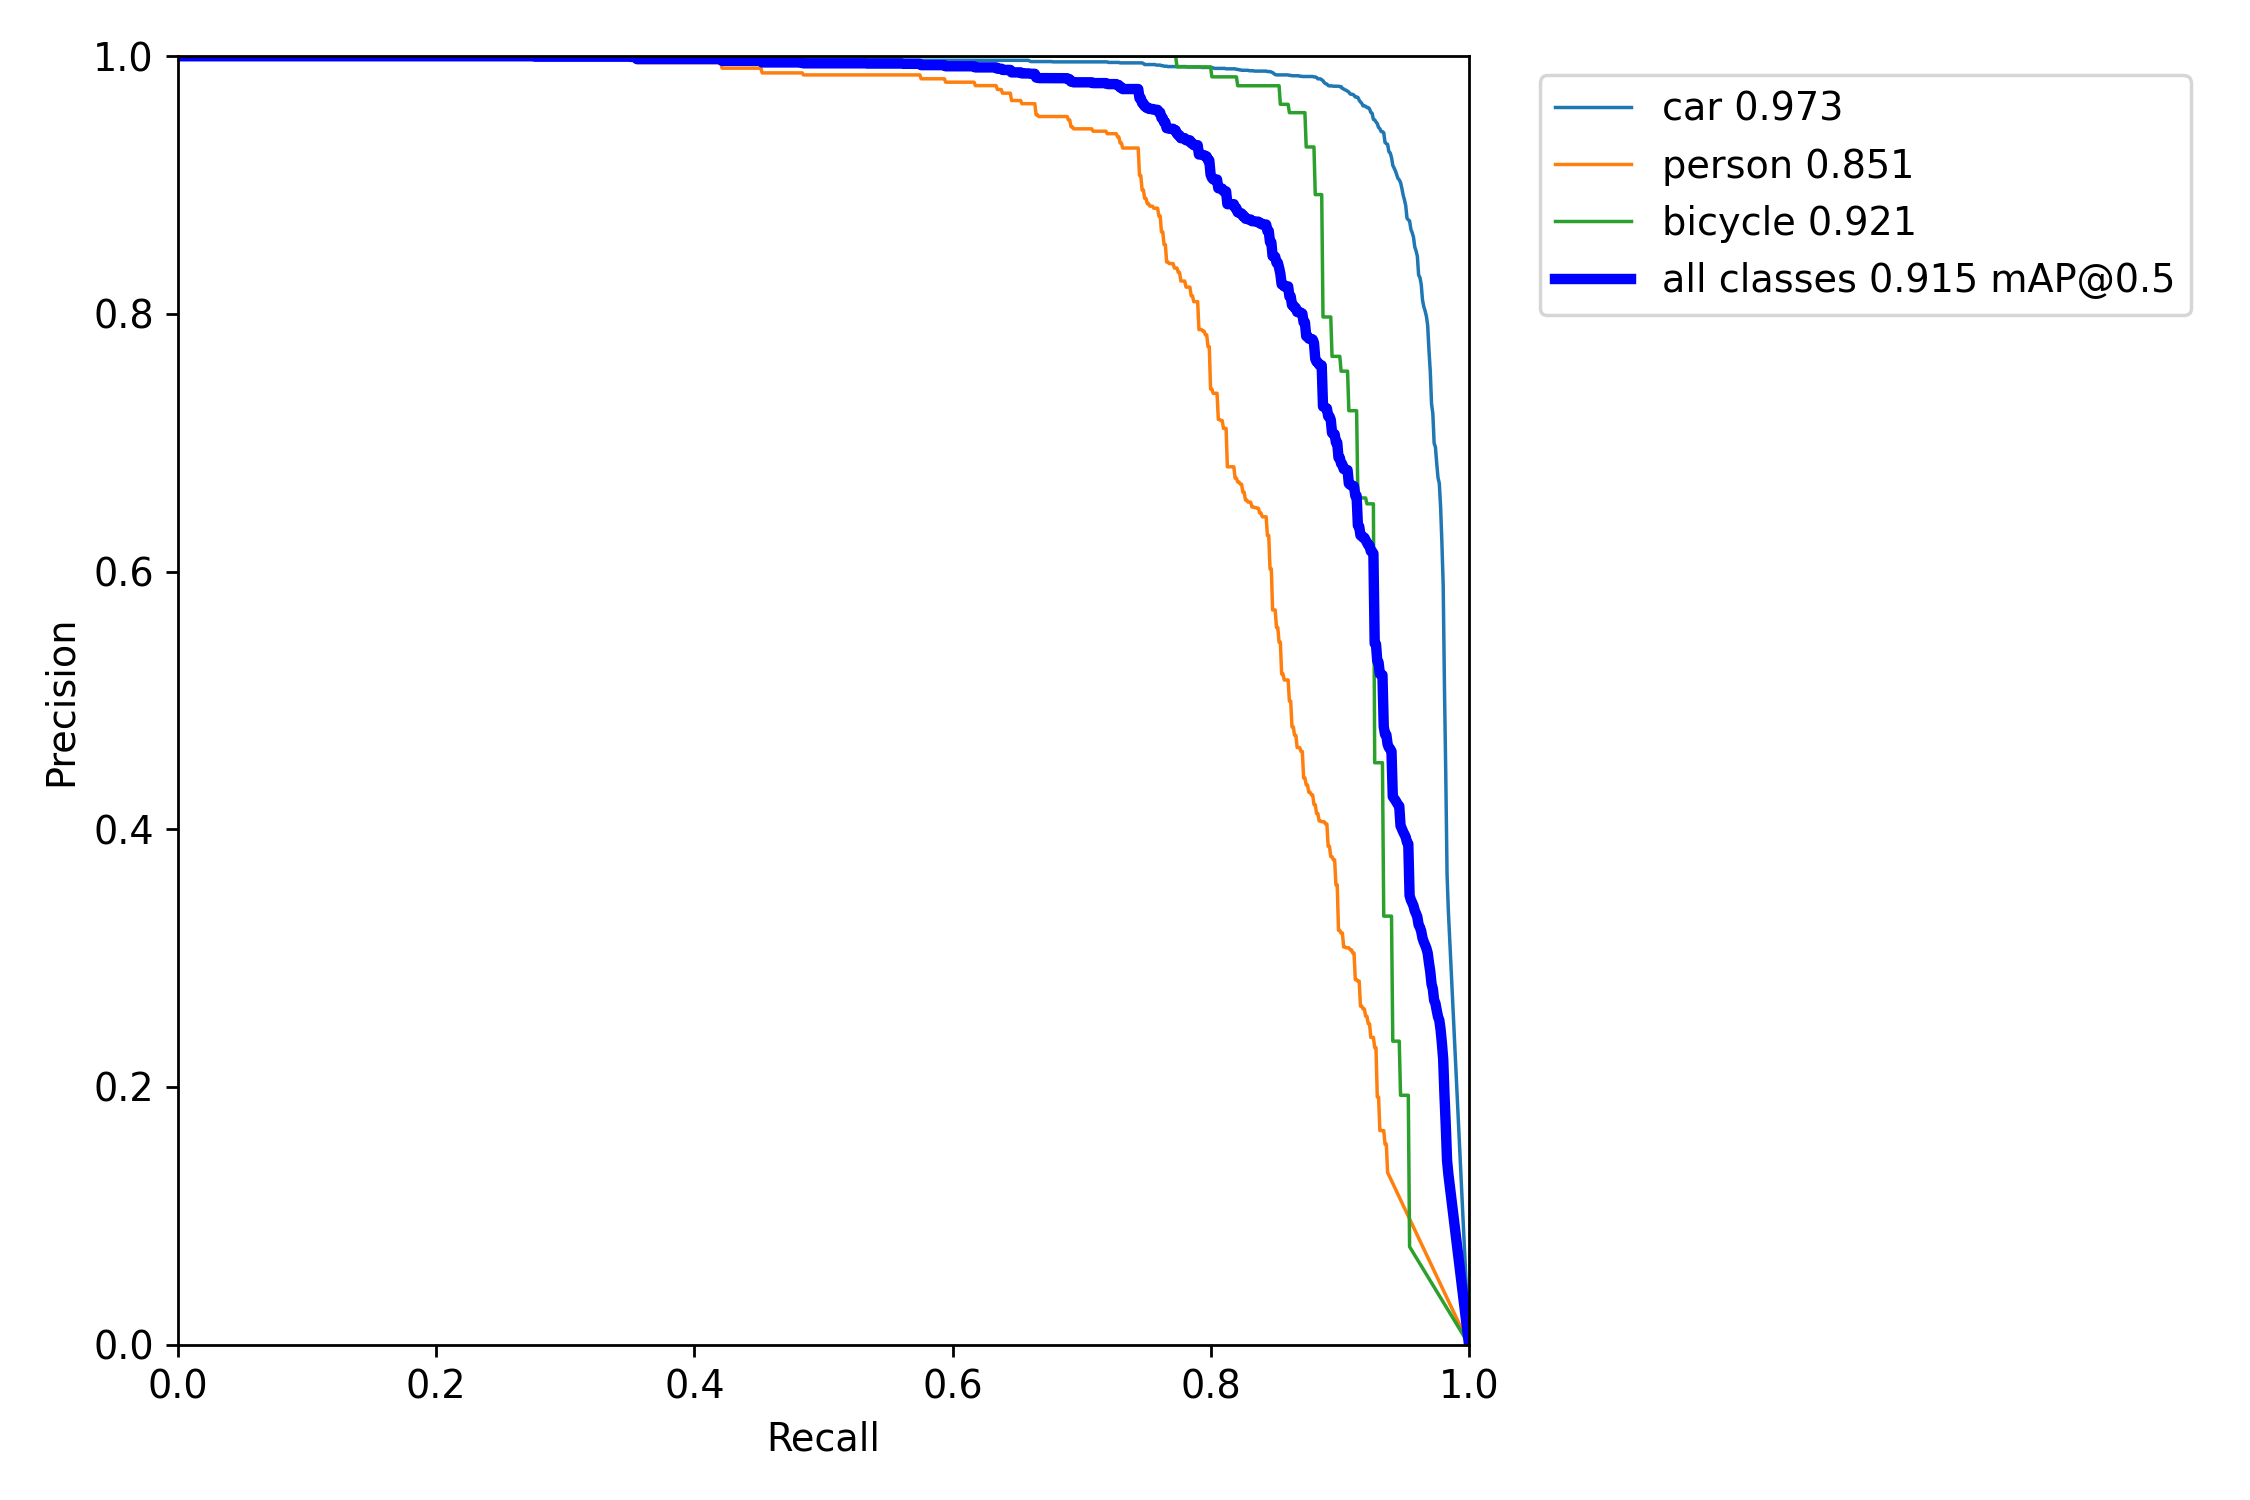
\includegraphics[width=0.65\textwidth]{Book/figures/5_deteccion2d/PR_curve_yolo5m_ft.png}
    \caption{Curva PR del modelo YOLOv5m aplicando FT sobre KITTI.}
    \label{fig:Curva PR del modelo YOLOv5m aplicando FT sobre KITTI.}
\end{figure}

Habiendo decidido como modelo a utilizar aquel basado en YOLOv5m con los pesos obtenidos tras aplicar fine-tunning, se decide estudiar en profundidad la precisión del modelo elegido mediante la curva de \ac{PR} la cual se muestra en la Figura \ref{fig:Curva PR del modelo YOLOv5m aplicando FT sobre KITTI.}. En esta imagen se observa como aquellos objetos que son más grandes como los coches son más fáciles de detectar que aquellos que son más pequeños como los peatones. En general se observa una gran diferencia en la precisión del modelo entre las clases 'coche' y 'ciclista', respecto a la clase 'peatón' que tiene una precisión notablemente inferior, lo cual es lógico por el número de píxeles que ocupan en las imágenes en promedio esta última clase.

\begin{table}[H]
\centering
\begin{tabular}{|cccc|}
\hline
Tamaño de la entrada & Tiempo pre-procesamiento & Tiempo inferencia & Tiempo NMS \\ \hline
(1, 3, 640, 640)     & 0.1 ms                   & 7.7 ms            & 0.6 ms     \\ \hline
\end{tabular}
\caption{Tiempos de ejecución del modelo YOLOv5m}
\label{tab:Tiempos de ejecución del modelo YOLOv5m}
\end{table}

Debido a que el tiempo de ejecución de los modelos es una tarea clave dentro de este trabajo al tratar de construir un sistema en tiempo real que se compone de múltiples modelo, se estudian el tiempo de ejecución del modelo YOLOv5 con los datos visibles en la Tabla \ref{tab:Tiempos de ejecución del modelo YOLOv5m}. Teniendo como entrada la dada por defecto en el modelo YOLOv5, siendo esta una imagen RGB de tamaño 640x640 píxeles, se puede ver como el tiempo del pre-procesamiento de la imagen es despreciable, la ejecución de la red neuronal es aquello que más tiempo requiere, pero es destacable como el proceso realizado por el algoritmo \ac{NMS} ocupa más de un 7\% del tiempo total de ejecución únicamente para la eliminación de las bounding boxes sobrantes, lo cual se ve claramente en la Figura \ref{fig:Pasos realizados por YOLO}.

\begin{figure}[H]
	\begin{minipage}{0.495\textwidth}
		\centering
		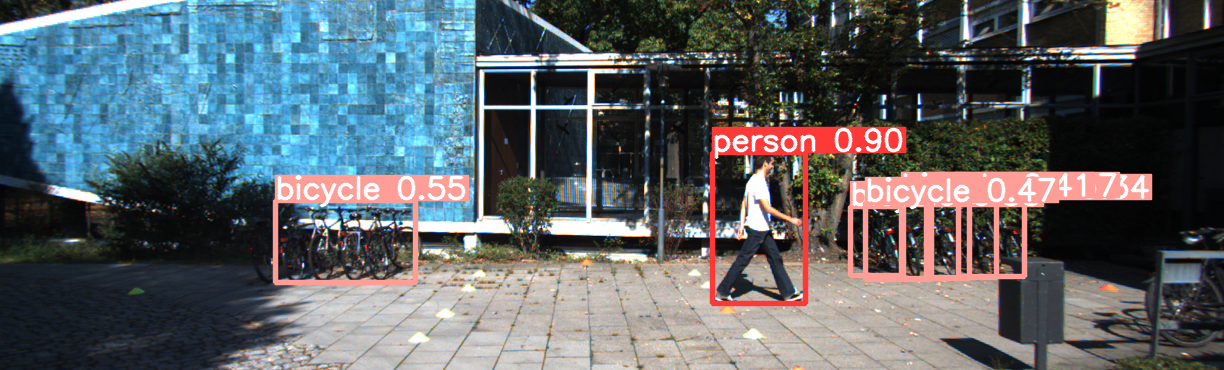
\includegraphics[width=1\linewidth]{Book/figures/5_deteccion2d/yolo_coco_0.png}
	\end{minipage}\hfill
	\begin{minipage}{0.495\textwidth}
		\centering
		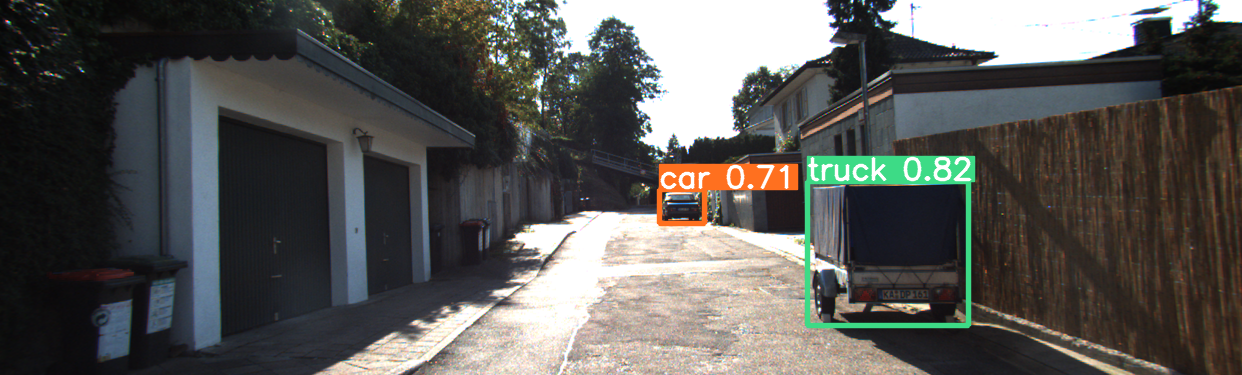
\includegraphics[width=1\linewidth]{Book/figures/5_deteccion2d/yolo_coco_1.png}
	\end{minipage}
	\caption{Detecciones de YOLOv5m con pesos entrenados sobre COCO.}
	\label{fig:Detecciones de YOLOv5m con pesos entrenados sobre COCO.}
\end{figure}

\begin{figure}[H]
	\begin{minipage}{0.495\textwidth}
		\centering
		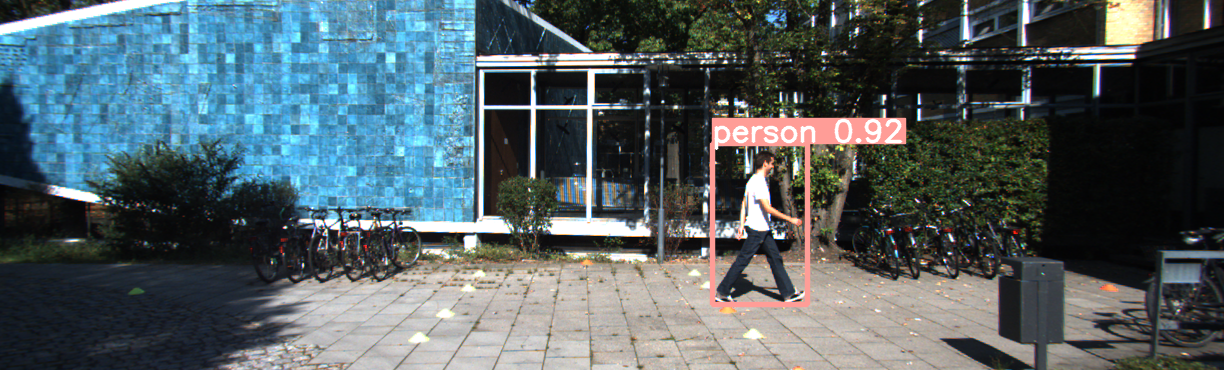
\includegraphics[width=1\linewidth]{Book/figures/5_deteccion2d/yolo_kitti_0.png}
	\end{minipage}\hfill
	\begin{minipage}{0.495\textwidth}
		\centering
		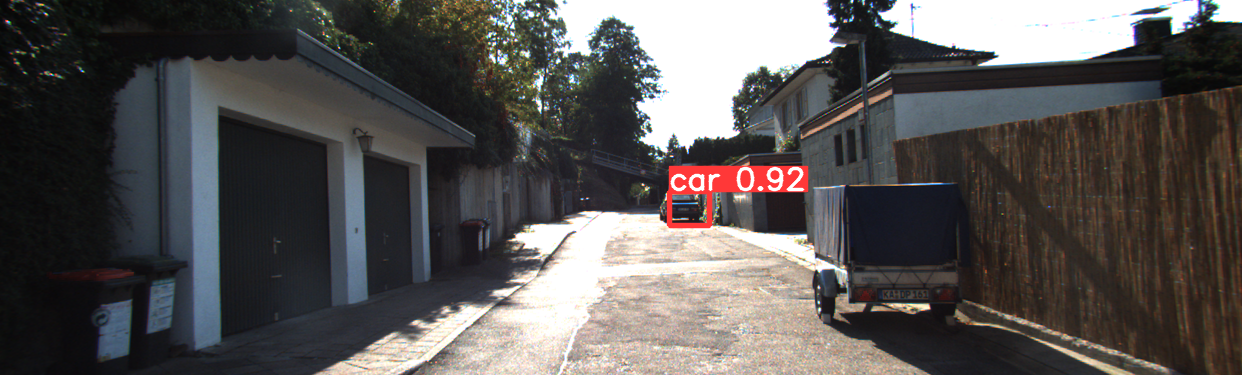
\includegraphics[width=1\linewidth]{Book/figures/5_deteccion2d/yolo_kitti_1.png}
	\end{minipage}
	\caption{Detecciones de YOLOv5m con pesos ajustados sobre KITTI.}
	\label{fig:Detecciones de YOLOv5m con pesos ajustados sobre KITTI.}
\end{figure}

Por último, se observan varios casos concretos dentro del dataset de KITTI para analizar de forma cualitativa la diferencia entre el uso del modelo YOLOv5m con los pesos entrenados sobre el dataset de COCO y el dataset de KITTI, para ello se atenderá a las Figuras \ref{fig:Detecciones de YOLOv5m con pesos entrenados sobre COCO.} y \ref{fig:Detecciones de YOLOv5m con pesos ajustados sobre KITTI.} donde se muestran las detecciones obtenidas con ambas redes. En estas imágenes se puede observar como: en el modelo entrenado sobre KITTI se obtienen únicamente las clases definidas para su detección y no todas las clases que podrían ser detectadas, como en este caso el remolque la carretera, por otra parte, al haber utilizado estos mismo datos para su entrenamiento; el modelo entrenado tiene una certeza superior de que las detecciones obtenidas son correctas en comparación al uso del modelo con los pesos que fueron entrenados sobre COCO debido al entrenamiento con datos iguales a los utilizados para mostrar estos casos; además es destacable resaltar como en en la imagen de la izquierda de la Figura \ref{fig:Detecciones de YOLOv5m con pesos entrenados sobre COCO.}, se puede ver un grupo de bicicletas que son agrupadas bajo una misma detección, esto es debido a que si se tiene una puntuación muy baja de las detecciones individuales, el algoritmo \ac{NMS} tratará de unirlas para reducir el número de detecciones como se explicó previamente, por lo que con el uso de los pesos del modelo entrenado sobre KITTI los cuales tienen una puntuación superior, no se suele encontrar con este tipo de errores.